\chapter{Specification and Design} 
\label{chap2}
%%%%%%%%%%%%%%%%%%%%%%%%%%%%%%%%%%%%%%%%

%\section{Overview}
This chapter will first specify what the software is \textit{required to do} and then it will show \textit{how to do it}, that is the design rationale behind it. It will also give a general overview of the working of the system, how the data flows in the system etc.

%%%%%%%%%%%%%%%%%%%%%%%%%%%%%%%%%%%%%%%%%%%%%%%%%%%%%%%%%%%%%%%%%%
\section{User Requirements}
The software system should be able to register new users, using a number of ways like email-password and third-party service providers like Google, Facebook, and Twitter, etc. Users should be able to add and remove other users as their \textbf{Contacts} using their email addresses. The system should keep track of the location of the user by running a lightweight background service and update their location periodically in the Database Server. The system should update the location of the user's Contacts in real-time and show their location on the Map. If the device supports Augmented Reality, the user should be able to view the location of their Contacts in the real-world using AR. The system should also provide real-time in-app chatting capability so the users could be able to communicate easily with one another. An in-app chat-bot should also be included to help out users and to make their experience more efficient and enjoyable.

%Context Diagrams
%
%URD Diagrams

\section{Architecture}
Our Android app will use \textbf{Firebase Authentication} for the authentication of users. It will then use Android background services and location services to retrieve the latest location update of the user and store it in \textbf{Firebase Realtime Database}. It will also use \textbf{Google Maps SDK} to show user markers on the Map, where their contacts are located, by retrieving them from the Firebase Database. If the device supports Augmented Reality, it will also fetch the user's contact's location details and show them in the real-world using \textbf{ARCore} library.

On the coding level, we will use \textbf{model-view-presenter (MVP)} architecture in our android application as it is engineered to facilitate automated unit testing and improve the separation of concerns in the presentation logic \cite{MVP2018}, as shown in Figure \ref{fig:Model_View_Presenter_GUI_Design_Pattern}. In model-view-presenter:
\begin{description}
    \item[Model] defines the data to be displayed in the user interface.
    \item[View] passive interface to display data and pass-out events to the presenter.
    \item[Presenter] acts upon model and view by retrieving data and displaying it in view.
\end{description}

\begin{figure}
    \centering
        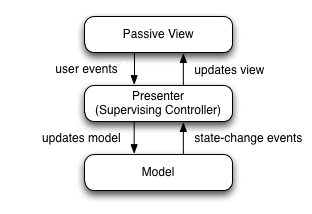
\includegraphics[width=0.50\textwidth]{images/Model_View_Presenter_GUI_Design_Pattern.png}
    \caption{Google MVP architecture}
    \label{fig:Model_View_Presenter_GUI_Design_Pattern}
\end{figure}


\section{Modules}
Separating the core logic of the application into different modules according to their functionality helps in managing, understanding and maintaining the code. Here we will briefly describe different modules being used by our application. 

The external modules that are being used extensively are:
\begin{description}[font=$\bullet$~, leftmargin=0cm]
    \item[FirebaseAuth] It provides the authentication functionality for the app. By using this, we could register, log-in and log-out a user from an active session. If the user is not authenticated, he will not be able to access the Firebase Database and as a result, will not be able to utilize this app.
    \item[FirebaseDatabase] This module provides functionality to read, write, update and delete data from the remote Firebase Database repository. We use this to update the user's information, location, contacts information, messages, etc.
    \item[FirebaseUI] This module allows us to quickly connect common UI elements to Firebase APIs without having to write so much boilerplate code\cite{FirebaseUI2018}.
    \item[ButterKnife] It generates the boilerplate code for us to bind fields and methods to Android views.
    \item[GoogleMap] This module provides all the functionality needed to work with device location, from periodic location look-ups to marker display on the map.
    \item[ARCore] It is used for implementing Augmented Reality features into the application.
\end{description}

We have also separated our code base into separate modules according to their functionality. Different modules being used in our application are:
\begin{description}[font=$\bullet$~, leftmargin=0cm]
    \item[Activities] All the android activities are stored in this module.
    \item[Common] The common functionality that is shared between different classes and modules.
    \item[Fragments] Different fragments that are used in the activities.
    \item[Models] POJOs (plain old java objects) which are used to read and write information to the Database, as well as Android views, is stored in this module.
    \item[Services] Services that run in the background.
\end{description}

%\section{User Interface}

\section{Data Flow}
To understand how a system works, it is necessary to understand the data flow of the system first. How the data is being passed from one system to another, how it is being transformed, and how it is being processed inside the system.
Here, we will show how the data flows in our application. 

In Figure \ref{fig:dfd0}, we show a Level-0 Data Flow Diagram which maps out the general flow of information between the system and the user. The user will be able to manage his/her account, add or remove users from his/her contact list and send his/her location updates from the device to the application where they will be stored. The application will provide the user with contact's information and update him/her periodically with the location updates of his/her contacts.
\begin{figure}
    \centering
        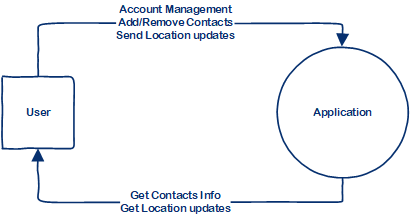
\includegraphics{images/dfd0.png}
    \caption{DFD Level 0}
    \label{fig:dfd0}
\end{figure}

In Level-1 DFD, Figure \ref{fig:dfd1}, we break down processes into further sub-processes to show how they interact with each other. There are several systems in our application that can act like standalone systems, like User Management System, Contact Management System, Location Tracking System etc. Here, we show how these systems interact with one another, how the user interacts with the system, and how different modules interact with the remote Firebase database.

\begin{figure}
    \centering
        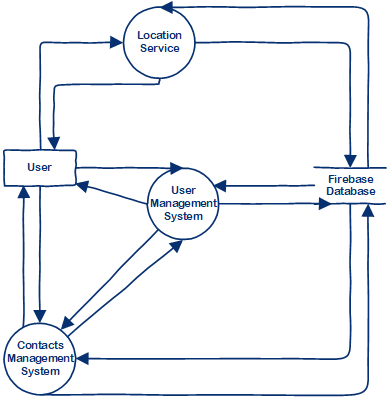
\includegraphics{images/dfd1.png}
    \caption{DFD Level 1}
    \label{fig:dfd1}
\end{figure}


\section{Data Schema} \label{data schema}
We are using Firebase Database, which is a \textbf{NoSQL database}. In a NoSQL database, data is modeled in means other than the tabular relations that are used in relational databases \cite{NoSQLWiki2018}. As compared to relational databases, NoSQL databases are more scalable, robust and provide superior performance. The data structures that are used by NoSQL databases (e.g., key-value, wide column, graph, or document) are different from those that are used by default in relational databases, making some operations faster in NoSQL.

Firebase Database is a NoSQL database that uses \textbf{JSON}. It has different optimizations and functionality compared to a relational database. It is a recommended practice to avoid nesting of data in Firebase DB because it might result in unnecessary data retrieval, e.g. if we want to get only the name of the user but our database schema is such that we have nested chat messages sent by that user into the user node, then it'll fetch all the messages as well, which is inefficient and a waste of network resources as well. So it is a best practice to avoid the nesting of data and only include as much as required for a particular scenario.

Another good practice is the denormalization of data, that is, data is split into separate paths. This helps in retrieving only the desired information at a particular time. For example, we might store chatting messages data in their separate nodes and location data in its separate node and user information in a separate node. When we need some specific data, we will be able to fetch only that.

Although Entity Relationship Diagram (ERD) is not a good fit for describing the schema of a NoSQL database, still we have provided it here, in Figure \ref{fig:erd}, to give you a general overview of what different fields are being stored and what is the relationship between them.

\begin{figure} [H]
    \centering
        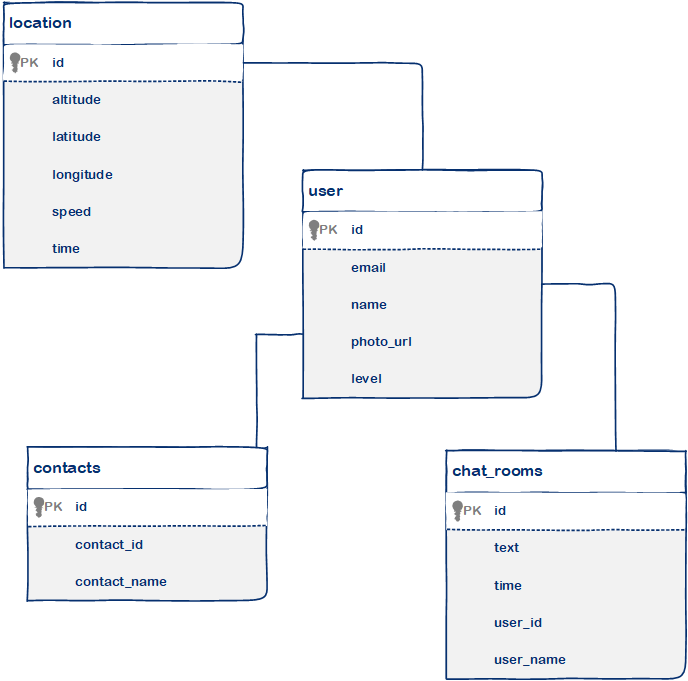
\includegraphics[width=0.75\textwidth]{images/erd.png}
    \caption{Entity Relationship Diagram}
    \label{fig:erd}
\end{figure}

Now, we will talk about how the data is being stored in the Firebase database as a JSON tree and how different fields are connected to one another. At the top level, we have four separate nodes for different kinds of data.
 
\begin{verbatim}
app 
{
    users: {}
    locations: {}
    contacts: {}
    chat_rooms: {}
}
\end{verbatim}

We will explain the structure of each and every node in further detail below, and show how we have followed best practices in defining the data schema for this project.

First of all, \texttt{users} node is used to store all the information about the user that is needed in the app.
\begin{verbatim}
"users" : {
    "tBEJnga0qOePwQhfhEVFP0uC1zB2" : {
      "email" : "aadimator@gmail.com",
      "name" : "Aadam",
      "photoUrl" : "https://link-to-photo/photo.jpg"
    }
}
\end{verbatim}
At first, we have the user id (UID), generated when he registers for the first time and stored here for future reference, that is used to identify the user throughout the application. Then we store basic information like his email id, his name and profile picture that we use in the application on various points.

\texttt{locations}, as the name suggests, is used to store the location of a particular user. 
\begin{verbatim}
"locations" : {
    "tBEJnga0qOePwQhfhEVFP0uC1zB2" : {
      "altitude" : 0,
      "latitude" : 33.9859268,
      "longitude" : 72.9703671,
      "speed" : 0,
      "time" : 1514393767560
    }
}
\end{verbatim}
The same \texttt{id} is used to store the location as the one used to store the user information in the \texttt{users} node. This helps in easy retrieval of relevant information.

\texttt{contacts} node is used to store the information about the contacts of a particular user.
\begin{verbatim}
"contacts" : {
    "tBEJnga0qOePwQhfhEVFP0uC1zB2" : {
        "4eTIfKSASHfSNjqv5rr1Ay3uKuS2" : "Panda",
              "xwykXzzlMjXJvNVjUbk65ZZxvjt2" : "Po"
    }
}
\end{verbatim}
We store the \texttt{uid} and \texttt{name} of the contact. We also store the name as it is mostly used in the application. The name of the contact is displayed in the list so instead of querying for full user information, we store his name here which reduces the number of queries to the database.

At the end, we have \texttt{chat\_rooms}. The \texttt{id} for the \texttt{chat\_rooms} node is generated by concatenating the two unique ids of the users that are participating in the current chat room. This ensures that it will always be unique and easily accessible.
\begin{verbatim}
"chat_rooms" : {
    "tBEJnga0qOePwQhfhEVFP0uC1zB2_oxCpx7sffgRfTc7SrLBTcW0LGW12" : {
        "-LI0dHZ6ff_GBJg3CNqO" : {
          "text" : "we are in the process of moving and I will",
          "time" : 1532257184164,
          "userId" : "oxCpx7sffgRfTc7SrLBTcW0LGW12",
          "userName" : "Po"
        },
        "-LI0eJcQzi6yx8Qn45Hl" : {
          "text" : "thanks for understanding",
          "time" : 1532257454754,
          "userId" : "tBEJnga0qOePwQhfhEVFP0uC1zB2",
          "userName" : "Aadam"
        }
        }
}
\end{verbatim}
In the \texttt{userId} and \texttt{userName}, we store the details of the user that is sending that particular message.

By looking at this Data Schema, you can see how we followed best practices, that is, avoided nesting of data and tried to denormalized the data. Each separate path or node serves a particular purpose and only contains information for a specific scenario.

\begin{figure}[H]
	\centering
		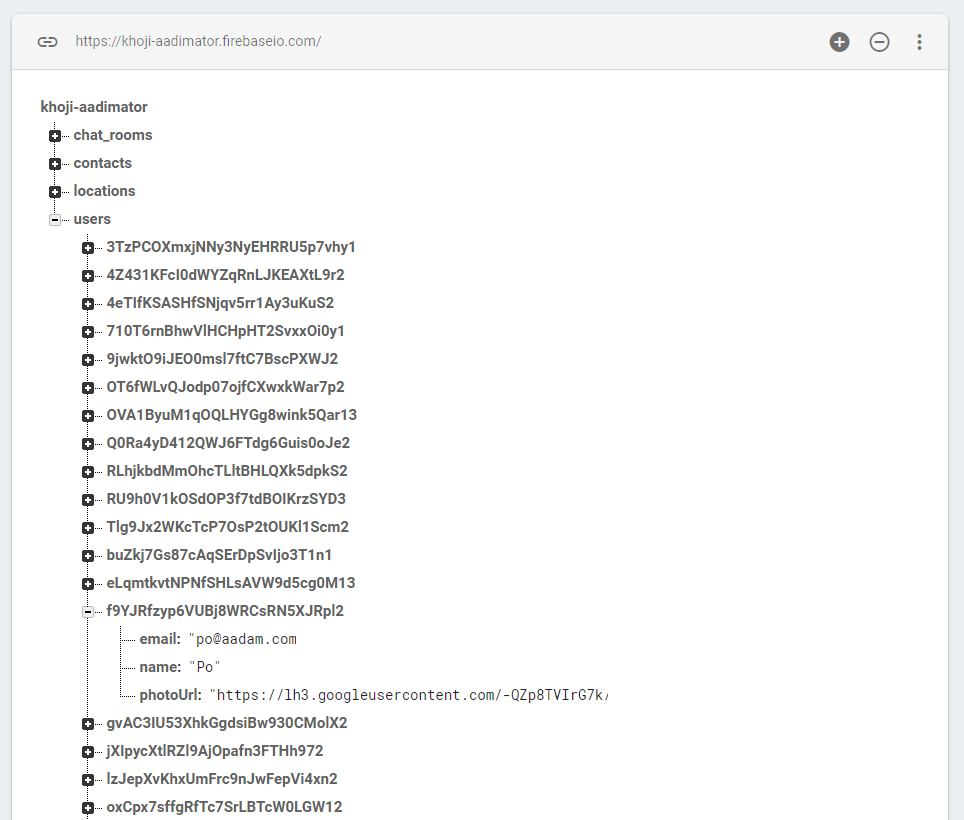
\includegraphics[width=1.00\textwidth]{images/khoji_firebase_db.PNG}
	\caption{Firebase Database of our system}
	\label{fig:khoji_firebase_db}
\end{figure}


\section{Design and Implementation Constraints}
One of the major constraints is the availability of the internet. Although we have enabled offline persistence in our application, which will store the data locally in case of network failure and upload it immediately when the network is back on, the real-time nature of the app will be affected by the unavailability of a network connection.

Another thing to keep in mind is the Firebase Database Limits \cite{FirebaseUsageLimits2018}. Although we can scale up to a bigger tier, it will cost more and given that one of the primary objectives of this project was to be more economical, we have to design our system accordingly.

We also have to keep in mind those users who do not have a compatible device for Augmented Reality features. We want to design our app in such a way that it is still accessible and usable for those users as well. If we only design for users with Augmented Reality supported devices, it would significantly reduce our user-base, thus affecting the usability of the app because most of the users will not be able to add their friends or family as their contacts.

We also have to keep in mind the background services constraint that has been implemented in Android v8.0 and above. Now, the apps can not use background services as frequently as they want but some time and frequency constraints are applied to them. Once the app is in the background, it can only listen for background updates a few times in an hour. This is used to improve the battery performance of the smartphone. 







